%!TEX root = ../tesis.tex

\chapter{Segundo capítulo}

\section{Una sección importante}

\begin{enumerate}
	\item The first topic is dull
	\item The second topic is duller
	\begin{enumerate}
		\item The first subtopic is silly
		\item The second subtopic is stupid
	\end{enumerate}
	\item The third topic is the dullest
\end{enumerate}
\begin{itemize}
	\item The first topic is dull
	\item The second topic is duller
	\begin{itemize}
		\item The first subtopic is silly
		\item The second subtopic is stupid
	\end{itemize}
	\item The third topic is the dullest
\end{itemize}

\begin{description}
\item[The first topic] is dull
\item[The second topic] is duller
\begin{description}
\item[The first subtopic] is silly
\item[The second subtopic] is stupid
\end{description}
\item[The third topic] is the dullest
\end{description}

\section{Otra sección} \label{sec:otra_seccion}

Una referencia a la \autoref{fig:plot}, dentro del \autoref{sec:otra_seccion}.

\begin{figure}[h]
	\centering
	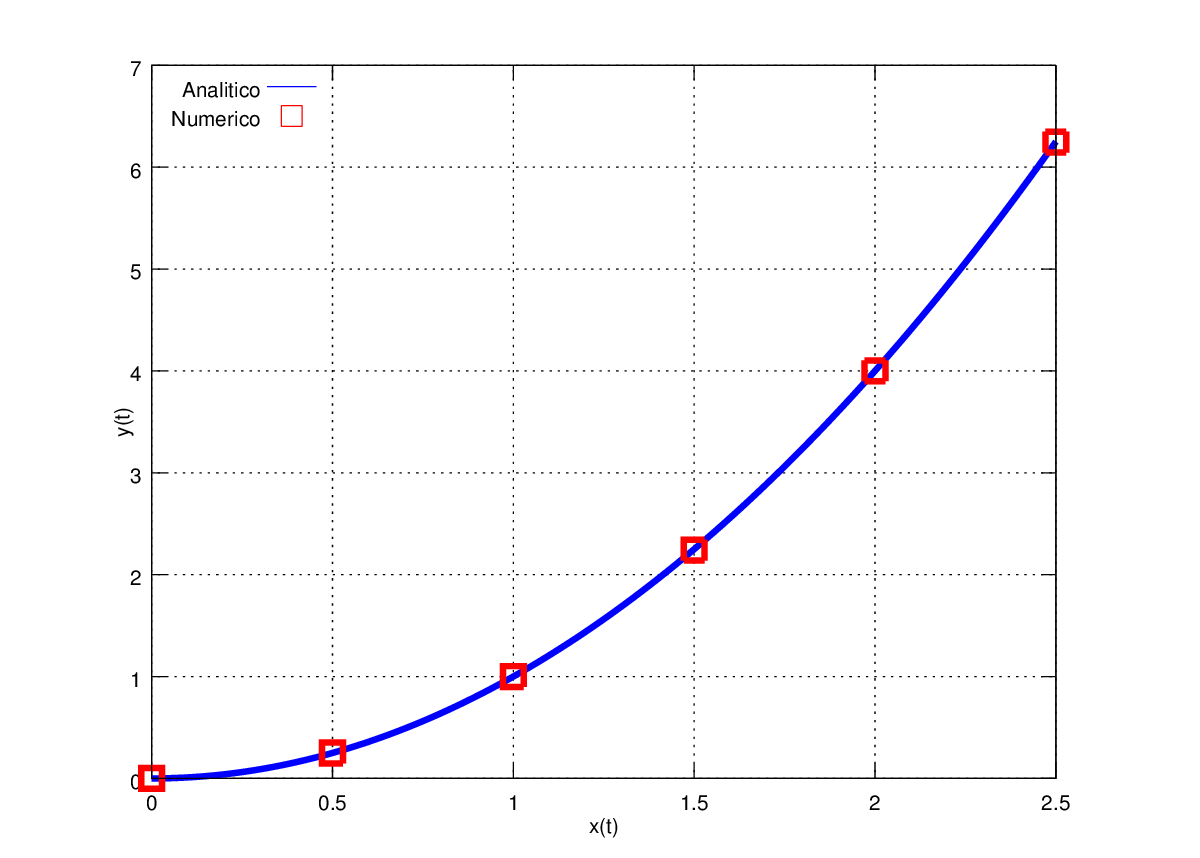
\includegraphics[width=0.7\textwidth]{Figuras/capitulo_2/x_vs_y}
	\caption{Gráfico de ejemplo.}
	\label{fig:plot}
\end{figure}

